\section{Evolution of Particle Surfaces by Node Shifting}\label{sec:surface-evolution}

\begin{figure}
    \begin{subfigure}{\linewidth}
        \centering
        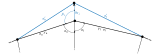
\includegraphics{img/model_development/node_shift_normal}
        \caption{Normal Direction}
        \label{fig:model_development/surface_normal}
    \end{subfigure}
    \begin{subfigure}{\linewidth}
        \centering
        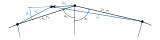
\includegraphics{img/model_development/node_shift_tangential}
        \caption{Tangential Direction}
        \label{fig:model_development/surface_tangential}
    \end{subfigure}
    \caption{Shifting of Surface Nodes}
    \label{fig:surface-node-shifting}
\end{figure}

\begin{figure}
    \begin{subfigure}{0.5\linewidth}
        \centering
        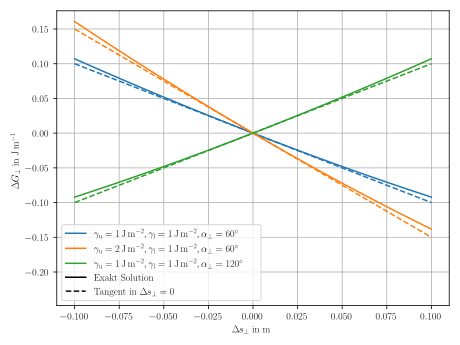
\includegraphics[scale=0.5]{img/model_development/plot_normal_potential}
        \caption{Normal Direction}
        \label{fig:model_development/plot_normal_potential}
    \end{subfigure}%
    \begin{subfigure}{0.5\linewidth}
        \centering
        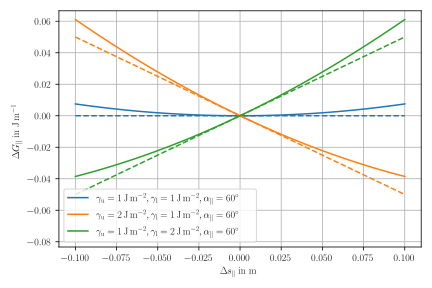
\includegraphics[scale=0.5]{img/model_development/plot_tangential_potential}
        \caption{Tangential Direction}
        \label{fig:model_development/plot_tangential_potential}
    \end{subfigure}
    \caption{Change in Gibbs Energy Due to Node Shifting (tangents dashed)}
    \label{fig:surface-node-potentials}
\end{figure}

In the following, the Gibbs energy and volume gradients when shifting nodes will be derived as needed in the formulation of dissipation $\Dissipation$ and dissipation function $\DissipationFunction$ given above.

\subsection{Normal Shifting}

The main mode of node shifting on free surfaces and grain boundaries is along the interface normal vector.
\autoref{fig:model_development/surface_normal} shows the principal geometry of a surface node and it's normal mode of shifting.

If a node is displaced in space, a change in Gibbs energy occurs due to the change in surface respectively interface area.
The amount of energy bound in a surface or interface is described by the interface energy $\InterfaceEnergy$.
Since a 2D problem is regarded, the length of the surface line $\SurfaceDistance$ is a measure of present surface area.
The change of Gibbs energy due to normal node shifting is described by \autoref{eq:gibbs-diff-surface-normal} with the prime values as measures after shifting.
\begin{equation}
    \Step\GibbsEnergy_{\Normal} = \left( \SurfaceDistance_{\Upper}' - \SurfaceDistance_{\Upper} \right) \InterfaceEnergy_{\Upper} +  \left(\SurfaceDistance_{\Lower}' - \SurfaceDistance_{\Lower} \right) \InterfaceEnergy_{\Lower}
    \label{eq:gibbs-diff-surface-normal}
\end{equation}

The normal vector points under an angle of $\SurfaceVectorAngle_\Normal$ acc.~to~\autoref{eq:delta-surface-normal} to both surface lines.
\begin{equation}
    \SurfaceVectorAngle_{\Normal} = \PI - \frac{1}{2} \left(\SurfaceRadiusAngle_{\Upper} + \SurfaceRadiusAngle_{\Lower} \right)
    \label{eq:delta-surface-normal}
\end{equation}

With a certain normal shift ${\Step\Shift}_\Normal$, the surface lengths after shifting are calculated by \autoref{eq:surface-distance-shifted-normal}.
\begin{subequations}
    \begin{align}
        \SurfaceDistance_{\Upper}' & = \sqrt{\SurfaceDistance_{\Upper}^2 + \Step\Shift_{\Normal}^2 - 2 \SurfaceDistance_{\Upper} \Step\Shift_{\Normal} \cos \SurfaceVectorAngle_{\Normal}} \label{eq:surface-distance-shifted-normal-upper}         \\
        \SurfaceDistance_{\Lower}' & = \sqrt{{\SurfaceDistance}_{\Lower}^2 + {\Step\Shift}_{\Normal}^2 - 2 {\SurfaceDistance}_{\Lower} {\Step\Shift}_{\Normal} \cos \SurfaceVectorAngle_{\Normal}} \label{eq:surface-distance-shifted-normal-lower}
    \end{align}
    \label{eq:surface-distance-shifted-normal}
\end{subequations}

\autoref{fig:model_development/plot_normal_potential} shows the change in Gibbs energy due to normal shifting with use of \autoref{eq:gibbs-diff-surface-normal} to \autoref{eq:surface-distance-shifted-normal} with different values of $\SurfaceVectorAngle_{\Normal}$ and $\InterfaceEnergy$, alongside the linear approximation around ${\Step\Shift}_{\Normal} = 0$.
Note, that the slope is dependent on the sum of ${\InterfaceEnergy}_{\Upper}$ and ${\InterfaceEnergy}_{\Lower}$ and the sign is only dependent on $\SurfaceVectorAngle_{\Normal}$.
$\SurfaceVectorAngle_{\Normal} > \qty{90}{\degree}$ means a convex surface, thus energy gain when inward shifting (negative ${\Step\Shift}_{\Normal}$).
$\SurfaceVectorAngle_{\Normal} < \qty{90}{\degree}$ means a concave surface, thus energy gain when outward shifting (positive ${\Step\Shift}_{\Normal}$).
$\SurfaceVectorAngle_{\Normal} = \qty{90}{\degree}$ means an even surface, thus energy loss in both shifting directions.

The partial derivative of Gibbs energy is obtained as the limit of $\Step\GibbsEnergy_{\Normal}$ when ${\Step\Shift}_{\Normal} \rightarrow 0$ as in \autoref{eq:gibbs-partial-surface-normal}.
\begin{equation}
    \frac{\partial \GibbsEnergy}{\partial {\Shift}_{\Normal}} = \lim_{\Step\Shift_{\Normal} \rightarrow 0} \frac{\Step\GibbsEnergy_{\Normal}}{\Step\Shift_{\Normal}} = -\left({\InterfaceEnergy}_{\Upper} + {\InterfaceEnergy}_{\Lower}\right) \cos \SurfaceVectorAngle_{\Normal}
    \label{eq:gibbs-partial-surface-normal}
\end{equation}

The volume derivative is obtained by calculating the area of the triangles formed by $\SurfaceDistance$, $\SurfaceDistance'$ and $\Step\Shift_{\Normal}$ on the upper and lower side.
\begin{subequations}
    \begin{align}
        \Step\Volume_{\Normal\Upper} &= \frac12 \SurfaceDistance_{\Upper} \Step\Shift_{\Normal} \sin \SurfaceVectorAngle_{\Normal} \\
        \Step\Volume_{\Normal\Lower} &= \frac12 \SurfaceDistance_{\Lower} \Step\Shift_{\Normal} \sin \SurfaceVectorAngle_{\Normal}
    \end{align}
    \label{eq:volume-diff-surface-normal}
\end{subequations}

The partial derivative of volume is obtained as the limit of $\Step\Volume_{\Normal\Upper} + \Step\Volume_{\Normal\Lower}$ when ${\Step\Shift}_{\Normal} \rightarrow 0$ as in \autoref{eq:volume-partial-surface-normal}.
\begin{equation}
    \frac{\partial \Volume}{\partial {\Shift}_{\Normal}} = \lim_{\Step\Shift_{\Normal} \rightarrow 0} \frac{\Step\Volume_{\Normal\Upper} + \Step\Volume_{\Normal\Lower}}{\Step\Shift_{\Normal}} = \frac{1}{2} \left( \SurfaceDistance_{\Upper} + \SurfaceDistance_{\Lower} \right) \sin \SurfaceVectorAngle_{\Normal}
    \label{eq:volume-partial-surface-normal}
\end{equation}

\subsection{Tangential Shifting}

Regarding the tangential shifting, the direction vector is under an angle of $\SurfaceVectorAngle_{\Tangential}$ acc.~to.~\autoref{eq:delta-surface-tangential} to the upper surface line.
\begin{equation}
    \SurfaceVectorAngle_{\Tangential} = \SurfaceVectorAngle_{\Normal} - \frac{\PI}{2}
    \label{eq:delta-surface-tangential}
\end{equation}

The change in Gibbs energy is calculated similarly as in the normal case according to \autoref{eq:gibbs-diff-surface-tangential}, but the shifted surface lengths are calculated as in \autoref{eq:surface-distance-shifted-tangential} in dependence on the tangential shift ${\Step\Shift}_{\Tangential}$.
Note especially the signs in front of the cosine terms.
\begin{equation}
    \Step\GibbsEnergy_{\Tangential} = \left( \SurfaceDistance_{\Upper}' - \SurfaceDistance_{\Upper} \right) \InterfaceEnergy_{\Upper} +  \left(\SurfaceDistance_{\Lower}' - \SurfaceDistance_{\Lower} \right) \InterfaceEnergy_{\Lower}
    \label{eq:gibbs-diff-surface-tangential}
\end{equation}
\begin{subequations}
    \begin{align}
        \SurfaceDistance_{\Upper}' & = \sqrt{{\SurfaceDistance}_{\Upper}^2 + {\Step\Shift}_{\Tangential}^2 - 2 {\SurfaceDistance}_{\Upper} {\Step\Shift}_{\Tangential} \cos \SurfaceVectorAngle_{\Tangential}} \label{eq:surface-distance-shifted-tangential-upper} \\
        \SurfaceDistance_{\Lower}' & = \sqrt{{\SurfaceDistance}_{\Lower}^2 + {\Step\Shift}_{\Tangential}^2 + 2 {\SurfaceDistance}_{\Lower} {\Step\Shift}_{\Tangential} \cos \SurfaceVectorAngle_{\Tangential}} \label{eq:surface-distance-shifted-tangential-lower}
    \end{align}
    \label{eq:surface-distance-shifted-tangential}
\end{subequations}

\autoref{fig:model_development/plot_tangential_potential} shows the change in Gibbs energy due to tangential shifting with different values of $\InterfaceEnergy$.
The slope and monotonicity of these curves is here dependent on the \emph{difference} of ${\InterfaceEnergy}_{\Upper}$ and ${\InterfaceEnergy}_{\Lower}$.
The convexity or concavity of the surface is here only of minor importance.
Whether the interface with higher $\InterfaceEnergy$ is located on the upper or lower side determines the monotonicity of the curves.
In the special case when ${\InterfaceEnergy}_{\Upper} = {\InterfaceEnergy}_{\Lower}$, the curve has a minimum in ${\Step\Shift}_{\Tangential} = 0$, meaning that any shift will produce an energy loss.
This is the case on all nodes except neck nodes.

Again, the partial derivative of Gibbs energy is found by the limit when ${\Step\Shift}_{\Tangential} \rightarrow 0$.
\begin{equation}
    \frac{\partial \GibbsEnergy}{\partial {\Shift}_{\Tangential}} = \lim_{\Step\Shift_{\Tangential} \rightarrow 0} \frac{\Step\GibbsEnergy_{\Tangential}}{\Step\Shift_{\Tangential}} = -\left({\InterfaceEnergy}_{\Upper} - {\InterfaceEnergy}_{\Lower}\right) \cos \SurfaceVectorAngle_{\Tangential}
    \label{eq:gibbs-partial-surface-tangential}
\end{equation}

The partial derivative of volume is found similarly as in the normal case, but the contribution of the lower side must be here counted negatively, as can be seen from \autoref{fig:model_development/surface_tangential}.
\begin{equation}
    \frac{\partial \Volume}{\partial {\Shift}_{\Tangential}} = \lim_{\Step\Shift_{\Tangential} \rightarrow 0} \frac{\Step\Volume_{\Tangential\Upper} - \Step\Volume_{\Tangential\Lower}}{\Step\Shift_{\Tangential}} = \frac{1}{2} \left( \SurfaceDistance_{\Upper} - \SurfaceDistance_{\Lower} \right) \sin \SurfaceVectorAngle_{\Tangential}
    \label{eq:volume-partial-surface-tangential}
\end{equation}

\subsection{Special Treatment of Neck Nodes}

\begin{figure}
    \begin{subfigure}{\linewidth}
        \centering
        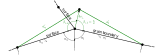
\includegraphics{img/model_development/node_shift_normal_neck}
        \caption{Normal Direction}
        \label{fig:model_development/node_shift_normal_neck}
    \end{subfigure}
    \begin{subfigure}{\linewidth}
        \centering
        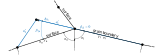
\includegraphics{img/model_development/node_shift_tangential_neck}
        \caption{Tangential Direction}
        \label{fig:model_development/node_shift_tangential_neck}
    \end{subfigure}
    \caption{Shifting of Neck Nodes}
    \label{fig:surface-node-shifting-neck}
\end{figure}

The neck nodes (triple points between two surfaces and one grain boundary) are a special case.
For numerical reasons, their shifting is not taken normal and tangential to the surface line, but only to the grain boundary, as this is in consistence with their primary evolution during sintering.
The case, where the grain boundary is located below the currently regarded node, is shown in \autoref{fig:surface-node-shifting-neck}.
Here, one must distinguish between the shift vector angles $\SurfaceVectorAngle$ to the upper and the lower surface line.
For the shown case the angles are as in \autoref{eq:shift-neck-angles}, if the grain boundary is, however, located above the node, than the values of the upper and lower angles have to be switched.
\begin{align}
    \SurfaceVectorAngle_{\Normal\Upper} = \frac32 \PI - \SurfaceRadiusAngle_{\Upper} - \SurfaceRadiusAngle_{\Lower} \qquad &\text{and} \qquad \SurfaceVectorAngle_{\Normal\Lower} = \frac\PI2 \\
    \SurfaceVectorAngle_{\Tangential\Upper} = \PI - \SurfaceRadiusAngle_{\Upper} - \SurfaceRadiusAngle_{\Lower} \qquad &\text{and} \qquad \SurfaceVectorAngle_{\Tangential\Lower} = 0
    \label{eq:shift-neck-angles}
\end{align}

The respective partial derivatives are slightly modified with the distinct angles as below.
\begin{align}
    \frac{\partial \GibbsEnergy}{\partial {\Shift}_{\Normal}} &= -\left( {\InterfaceEnergy}_{\Upper} \cos \SurfaceVectorAngle_{\Normal\Upper} - {\InterfaceEnergy}_{\Lower} \cos \SurfaceVectorAngle_{\Normal\Lower} \right)
    \label{eq:gibbs-partial-neck-normal} \\
    \frac{\partial \Volume}{\partial {\Shift}_{\Normal}} &= \frac{1}{2} \left( \SurfaceDistance_{\Upper} \sin \SurfaceVectorAngle_{\Normal\Upper} + \SurfaceDistance_{\Lower} \sin \SurfaceVectorAngle_{\Normal\Lower}\right)
    \label{eq:volume-partial-neck-normal} \\
    \frac{\partial \GibbsEnergy}{\partial {\Shift}_{\Tangential}} &= -\left( {\InterfaceEnergy}_{\Upper} \cos \SurfaceVectorAngle_{\Tangential\Upper} - {\InterfaceEnergy}_{\Lower} \cos \SurfaceVectorAngle_{\Tangential\Lower}\right)
    \label{eq:gibbs-partial-neck-tangential} \\
    \frac{\partial \Volume}{\partial {\Shift}_{\Tangential}} &= \frac{1}{2} \left( \SurfaceDistance_{\Upper} \sin \SurfaceVectorAngle_{\Tangential\Upper} - \SurfaceDistance_{\Lower} \sin \SurfaceVectorAngle_{\Tangential\Lower}\right)
    \label{eq:volume-partial-neck-tangential}
\end{align}
